\newcommand{\yeararrow}[4] {
	\draw[fill=#3, color=#3, inner sep = 0] (#1,#2) -- (#1+0.2,#2-0.2) -- (#1,#2-0.4)  -- (#1+1,#2-0.4) -- (#1+1.2,#2-0.2) -- (#1+1,#2) -- (#1,#2);
	\node[color=white] at (#1+0.6, #2-0.2) {#4};
}

\begin{addmargin}[0.05\textwidth]{0cm}
	\color{darkgray}
	\def\arraystretch{2} 
	\setlength\tabcolsep{0cm}
	\begin{tabular*}{0.9\textwidth}{l}
		\Large \faHourglass{ TIMELINE} \\ \Xhline{0.1cm}
	\end{tabular*}
	\color{darkgray}
	
	\vspace{0.5cm}
	
	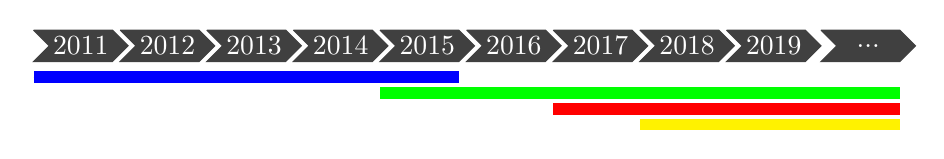
\begin{tikzpicture}
	\yeararrow{0}{0}{darkgray}{2011}
	\yeararrow{1.1}{0}{darkgray}{2012}
	\yeararrow{2.2}{0}{darkgray}{2013}
	\yeararrow{3.3}{0}{darkgray}{2014}
	\yeararrow{4.4}{0}{darkgray}{2015}
	\yeararrow{5.5}{0}{darkgray}{2016}
	\yeararrow{6.6}{0}{darkgray}{2017}
	\yeararrow{7.7}{0}{darkgray}{2018}
	\yeararrow{8.8}{0}{darkgray}{2019}
	\yeararrow{10}{0}{darkgray}{...}
	
	\draw[color=blue, fill=blue, line width=0.15cm] (5.4, -0.6) -- (0,-0.6);
	\draw[color=green, fill=blue, line width=0.15cm] (4.4, -0.8) -- (11,-0.8);
	\draw[color=red, fill=red, line width=0.15cm] (6.6, -1) -- (11,-1);
	\draw[color=yellow, fill=yellow, line width=0.15cm] (7.7, -1.2) -- (11,-1.2);
	\end{tikzpicture}
	
	\vspace{0.5cm}
	
	\color{darkgray}
	\def\arraystretch{2} 
	\setlength\tabcolsep{0cm}
	\begin{tabular*}{0.9\textwidth}{l @{\extracolsep{\fill} } p{0.8\textwidth}}
		\large \color{blue} \faSquare & \large Gymnasium Kraljevo, Department of Natural Sciences \\ \Xhline{0.05cm}
		\large \color{green} \faSquare & \large University of Belgrade, Faculty of Mathematics \newline Bachelor studies - Informatics \\ \Xhline{0.05cm}
		\large \color{red} \faSquare & \large OpenGL C++ 3D game project \newline https://github.com/MATF-RG18/RG146-vitez-reda-zmaja \\ \Xhline{0.05cm}
		\large \color{yellow} \faSquare & \large Syntax highlighter for Scintilla based text editors \newline https://github.com/pantelic-dusan/scintilla-scite \\ \Xhline{0.05cm}
	\end{tabular*}
	
\end{addmargin}